\documentclass[11pt]{article}
%\usepackage{fullpage}
\usepackage{epic}
\usepackage{eepic}
\usepackage{paralist}
\usepackage{graphicx}
\usepackage{algorithm,algorithmic}
\usepackage{tikz}
\usepackage{xcolor,colortbl}
\usepackage{wrapfig}


%%%%%%%%%%%%%%%%%%%%%%%%%%%%%%%%%%%%%%%%%%%%%%%%%%%%%%%%%%%%%%%%
% This is FULLPAGE.STY by H.Partl, Version 2 as of 15 Dec 1988.
% Document Style Option to fill the paper just like Plain TeX.

\typeout{Style Option FULLPAGE Version 2 as of 15 Dec 1988}

\topmargin 0pt
\advance \topmargin by -\headheight
\advance \topmargin by -\headsep

\textheight 8.9in

\oddsidemargin 0pt
\evensidemargin \oddsidemargin
\marginparwidth 0.5in

\textwidth 6.5in
%%%%%%%%%%%%%%%%%%%%%%%%%%%%%%%%%%%%%%%%%%%%%%%%%%%%%%%%%%%%%%%%

\pagestyle{empty}
\setlength{\oddsidemargin}{0in}
\setlength{\topmargin}{-0.8in}
\setlength{\textwidth}{6.8in}
\setlength{\textheight}{9.5in}


\def\ind{\hspace*{0.3in}}
\def\gap{0.1in}
\def\bigap{0.25in}
\newcommand{\Xomit}[1]{}


\begin{document}

\setlength{\parindent}{0in}
\addtolength{\parskip}{0.1cm}
\setlength{\fboxrule}{.5mm}\setlength{\fboxsep}{1.2mm}
\newlength{\boxlength}\setlength{\boxlength}{\textwidth}
\addtolength{\boxlength}{-4mm}
\begin{center}\framebox{\parbox{\boxlength}{{\bf
CS 4820, Spring 2018 \hfill Homework 7, Problem 3}\\
% TODO: fill in your own name, netID, and collaborators
Name: \\
NetID: \\
Collaborators:
}}
\end{center}
\vspace{5mm}

{ \bf (3)} {\em (10 points)}
Consider a puzzle in which you are given an $n$-by-$n$
square grid, with an integer in the range $\{0,\ldots,4\}$
written inside each grid cell. You are asked to select a
subset $F$ of the edges of the grid, such that for each 
grid cell the number written inside the cell matches 
the number of elements of $F$ that belong to
the cell's boundary. The following figure shows an 
example of a puzzle and a valid solution to the puzzle.

\begin{center}
\begin{minipage}{0.3\textwidth}
  \begin{tikzpicture}
    \draw[black] (0,0) grid (6,4);
    \node at (0.5,0.5) {1};
    \node at (1.5,0.5) {4};
    \node at (2.5,0.5) {3};
    \node at (3.5,0.5) {3};
    \node at (4.5,0.5) {2};
    \node at (5.5,0.5) {0};
    \node at (0.5,1.5) {1};
    \node at (1.5,1.5) {3};
    \node at (2.5,1.5) {1};
    \node at (3.5,1.5) {2};
    \node at (4.5,1.5) {3};
    \node at (5.5,1.5) {2};
    \node at (0.5,2.5) {2};
    \node at (1.5,2.5) {2};
    \node at (2.5,2.5) {1};
    \node at (3.5,2.5) {1};
    \node at (4.5,2.5) {3};
    \node at (5.5,2.5) {2};
    \node at (0.5,3.5) {3};
    \node at (1.5,3.5) {2};
    \node at (2.5,3.5) {2};
    \node at (3.5,3.5) {3};
    \node at (4.5,3.5) {2};
    \node at (5.5,3.5) {1};
  \end{tikzpicture}
\end{minipage}
\hspace*{0.1\textwidth}
\begin{minipage}{0.3\textwidth}
  \begin{tikzpicture}
    \draw[black] (0,0) grid (6,4);
    \node at (0.5,0.5) {1};
    \node at (1.5,0.5) {4};
    \node at (2.5,0.5) {3};
    \node at (3.5,0.5) {3};
    \node at (4.5,0.5) {2};
    \node at (5.5,0.5) {0};
    \node at (0.5,1.5) {1};
    \node at (1.5,1.5) {3};
    \node at (2.5,1.5) {1};
    \node at (3.5,1.5) {2};
    \node at (4.5,1.5) {3};
    \node at (5.5,1.5) {2};
    \node at (0.5,2.5) {2};
    \node at (1.5,2.5) {2};
    \node at (2.5,2.5) {1};
    \node at (3.5,2.5) {1};
    \node at (4.5,2.5) {3};
    \node at (5.5,2.5) {2};
    \node at (0.5,3.5) {3};
    \node at (1.5,3.5) {2};
    \node at (2.5,3.5) {2};
    \node at (3.5,3.5) {3};
    \node at (4.5,3.5) {2};
    \node at (5.5,3.5) {1};
    \draw[line width=4pt,line cap=rect] (0,4) -- (2,4);
    \draw[line width=4pt,line cap=rect] (1,4) -- (1,0);
    \draw[line width=4pt,line cap=rect] (0,3) -- (1,3);
    \draw[line width=4pt,line cap=rect] (1,2) -- (2,2);
    \draw[line width=4pt,line cap=rect] (1,1) -- (2,1) -- (2,0);
    \draw[line width=4pt,line cap=rect] (1,0) -- (3,0) -- (3,2);
    \draw[line width=4pt,line cap=rect] (2,3) -- (3,3) -- (3,4) -- (4,4) -- (4,3) -- (5,3);
    \draw[line width=4pt,line cap=rect] (4,3) -- (4,2) -- (6,2) -- (6,4);
    \draw[line width=4pt,line cap=rect] (3,1) -- (5,1) -- (5,2);
    \draw[line width=4pt,line cap=rect] (4,0) -- (4,1);
  \end{tikzpicture}
\end{minipage}
\end{center}
Design a polynomial-time algorithm that, when given
such a puzzle, either outputs a valid solution or 
decides (correctly) that there is no valid solution.

\vskip \bigap

%% Your solution goes here.

\end{document}
